\chapter{Searching for phylogenetic signal in the output of a reference-free variant caller}
\label{ch:structured}
\newpage
\section{Introduction}

Genotyping a sample given a set of next generation sequencing reads is a common task in biology. However, genotyping accurately and sensitively can be difficult due to errors in sequencing reads \parencite{fox_accuracy_2014, pfeifer_next-generation_2017, wu_estimating_2017}. This problem is exacerbated when genotyping non-model organisms because they may lack a polished annotated genome and other prior information that is sometimes used in genotyping pipelines. Additionally, it may be difficult to reliably extract undamaged DNA from the sample material, compounding the error problem \parencite{da_fonseca_next-generation_2016}. Once obtained, these genotypes can be used for many things; detecting selection in a population, discovering genes and alleles that affect a particular phenotype, or comparing them to another population to attempt to understand their evolutionary history.

While accurate genotype calls are important for all these purposes, accurate detection of variation is difficult even with plenty of time, money, and other auxilliary resources available. Without a high-quality genome and a large number of reads, the task becomes much harder. However, several methods have been developed to call variants directly from sequencing reads, with no additional information necessary. These methods traditionally use de bruijn graphs to create contiguous sequences representing the genome, much like a genome assembly \parencite{leggett_reference-free_2014}. They also keep track of which samples the sequences in the graph came from; once the graph is completed, it is traversed to find bubble-like structures in the graph. These are locations where the sequences specific to different samples diverge briefly, then come back together. This indicates the presence of a single nucleotide polymorphism (SNP) or short insertion-deletion in one of the samples. Then, the sequences that differ can be extracted from the graph and aligned to a reference, if one exists \parencite{iqbal_novo_2012, uricaru_reference-free_2015}.

Reference-free methods do not necessarily need to use de-bruijn graphs, however. As de bruijn graphs can be computationally expensive to create, particularly in the amount of computational time and memory required, alternative approaches have also been proposed that utilize different data structures. One method uses an extension of the Burrows-Wheeler transform to find sample divergence in similar sets of reads \parencite{prezza_snps_2019}, another does so via k-mer counting \parencite{audano_mapping-free_2018}. These methods all operate under a common  principle: that clustering similar reads together and finding the points of divergence can reveal divergence between samples, even without a reference genome.

There are a variety of software packages that implement reference-free variant calling. One of the first developed is an extension of the Cortex assembler and is called cortex\_var \parencite{iqbal_novo_2012}. A more recent method called DiscoSNP++ was developed which doesn't require as much RAM or CPU and allows direct VCF output after mapping the predicted variants to a genome \parencite{peterlongo_discosnp_2017}. DiscoSNP++ has recently been updated to include a tool specifically for use with RAD-seq data rather than whole genome sequencing data \parencite{gauthier_discosnp-rad_2020}. The recently developed method, Kestrel, attempts to find variants without a graph and solely considers k-mer counts \parencite{audano_mapping-free_2018}, while eBWT2SNP \parencite{prezza_snps_2019} utilizes an extended Burrows-Wheeler transform of reads \parencite{mantaci_extension_2007}.

I previously called genotypes in the non-model organism \textit{Eucalyptus melliodora} using both out-of-the-box and custom methods to genotype leaves sampled across the tree \parencite{orr_phylogenomic_2020}. I leveraged the sample structure to estimate false positive rates for each step in the pipeline I used. When I began that work, the available reference-free methods were not sufficiently developed to call variants with the necessary accuracy I wanted to be confident in the results. Since then, the methods have undergone more development, so I was interested in whether they would work for the same data. In this appendix, I use the reference-free variant caller DiscoSNP++ \parencite{peterlongo_discosnp_2017} construct phylogenies to see whether the output calls capture the branching genetic structure of the tree. I also compare the output of the caller with the set of confident variants detected using the maximum likelihood approach described in \parencite{orr_phylogenomic_2020} and implemented with DeNovoGear \parencite{ramu_denovogear_2013}.

\section{Methods}

%adapted from /storage/2017-03-15-eucalyptus/2019-12-16-supplement/filter_steps/false-positive-rate
%scripts are in /storage/2017-03-15-eucalyptus/2020-10-05-disco
To obtain variants to compare to the variant set obtained in \cite{orr_phylogenomic_2020}, I ran the DiscoSNP++ program on the raw sequencing reads. DiscoSNP++ was run with the included run\_discoSnp++.sh shell script with the -G, -T, and -R flags set along with the pseudo-reference genome from \cite{orr_phylogenomic_2020}. This enables alignment of the detected variants to the reference and creation of a VCF from the aligned haplotypes and places k-mers from the reference in the graph to aid in variant calling.

To understand how each filtering step previously applied to this data affected the number of variants in this set, I applied 7 of 8 of these filters to the set of variants. Prior to these filters, however, I used BCFTools \parencite{li_statistical_2011} to remove any site which included a ``." genotype, since every sample is diploid; ``./." genotypes were permitted until the second to last step. The first filter only permits variants that appear on the first 11 scaffolds of the genome; these represent the chromosomes of \textit{E. melliodora}. Variants with depth > 500 were then excluded, as higher than expected depth is a signal of alignment problems. The ExcessHet annotation could not be used for filtering, as this filter is specific to GATK. I then filtered out variants within 50bp of an indel, another indicator of alignment issues. I then removed any variant that was not a biallelic SNP, as these are more likely to be errors than true mutations. Note that this makes it impossible for this pipeline to detect heterozygous to heterozygous mutations. I then removed variants that were in repetitive regions determined by a liftover of the \textit{E. grandis} RepeatMasker annotation \parencite{bartholome_high-resolution_2015} to the pseudo-reference. Finally, I removed all sites where any set of three replicates did not have the same genotype. I then included only sites that included a mutation (\textit{ie.} not all heterozygous) to get the final set of variants.

To visualize how each filtering step affected the overall quality of the called variants, I concatenated the variants found in each step to create a FASTA alignment of sites and used RAxML \parencite{stamatakis_raxml_2014} with the -f a option to search for the best-scoring maximum likelihood tree, the -m ASC\_GTRGAMMA model to use a GTR mixture model with gamma distributed rate heterogeneity and correct for ascertainment bias, and the -\phantom{}-asc-corr lewis option to use Lewis' correction for ascertainment bias \parencite{lewis_likelihood_2001}. Variant concatenation is not the optimal way to infer accurate phylogenies; however, for the purposes of a visual summary of the data it is sufficient. Trees were visualized in R \parencite{r_core_2020} with the ape package \parencite{paradis_ape_2019}.

I also compare the output calls to the set of confident set of mutation calls made in \cite{orr_phylogenomic_2020}. Note that, as found in \cite{orr_phylogenomic_2020}, this set has an approximate false negative rate of 30\%, so there are likely many real mutations in the output DiscoSNP++ calls that are not present in the confident call set.

Scripts to reproduce these analyses are shown in Appendix \ref{ch:evaluating_code}.

\section{Results}

DiscoSnp++ emitted a total of of 1,114,434 potential variants; however, only 951,924 of these mapped to one of the first 11 scaffolds. After applying all filters, only 4 variants were ultimately detected (see Table \ref{tbl:ev_num_variants}). Before filtering, 27 of the 90 possible confident set variants were detected; after filtering, none were.

\begin{table}
\begin{tabularx}{\textwidth}{X X X}
\toprule
\textbf{Description} & \textbf{Num \newline Variants} & \textbf{Previously Detected Variants}\\
\midrule
Appears in first 11 scaffolds & 951924 & 27\\
Total depth <= 500 & 910361 & 27\\
Not within 50bp of an indel & 893535 & 26\\
Biallelic SNPs & 815925 & 26\\
Outside repeat regions & 432414 & 20\\
All 3 replicates match & 2150 & 0\\
Only variable sites & 4 & 0\\
\bottomrule
\end{tabularx}
\titlecaption{Number of Detected Variants After Each Filtering Step}{The number of variants detected at each filtering step. Each row introduces a new filter that applies in addition to all the filters in the above rows. A description of each filter, the number of variants remaining after the filter has been applied, and the number of variants that overlap the previously estimated confident set of variants, which contains 90 variants, are shown.}
\label{tbl:ev_num_variants}
\end{table}

The trees inferred from the set of variants detected at each site are shown in Figure \ref{fig:ev_filtertrees}. The second to last filtering step where variants only pass filtering if they are consistent in all three replicates and the last filtering step where variants only pass filtering if there is a mutation (\textit{ie.} not all heterozygous sites of the same genotype) both yielded the same tree, as the nonvariable sites are removed in the tree construction pipeline. Each tree structure differs significantly from the true tree, and there are few examples of all three replicates neighboring one another.

\begin{figure}

\centering
\begin{tabularx}{.7\textwidth}{ >{\hsize=.7\hsize\linewidth=\hsize}X >{\hsize=1.3\hsize\linewidth=\hsize}X}
\toprule
Filtering Step & Tree \\
\midrule
First 11 Scaffolds & 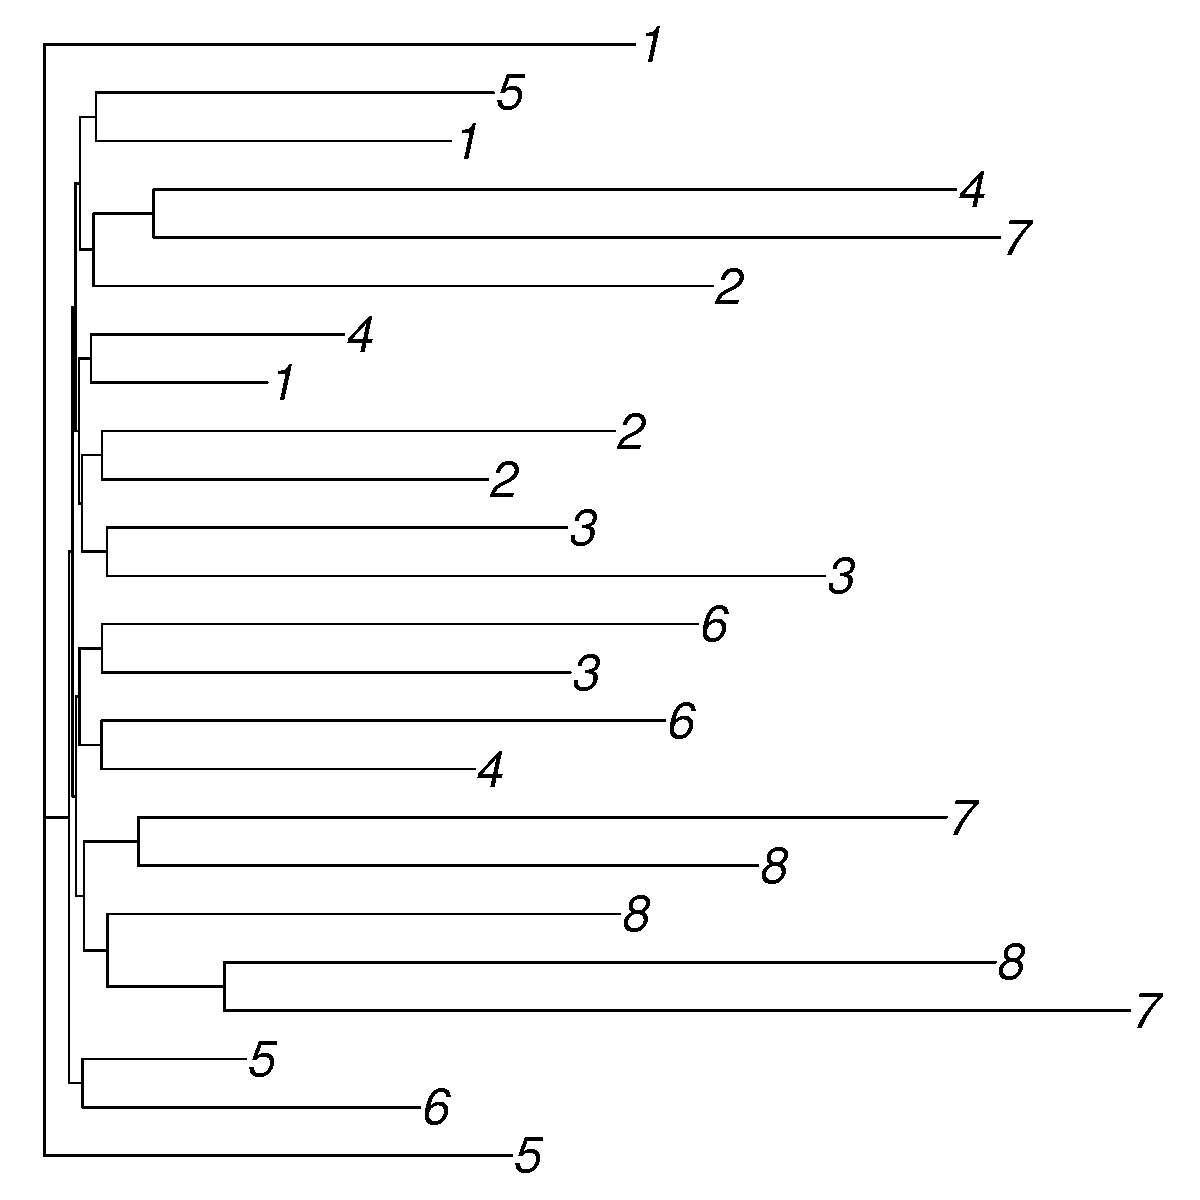
\includegraphics[width=.9\linewidth]{01-first-11-scaffolds.pdf} \\
Depth <= 500 & 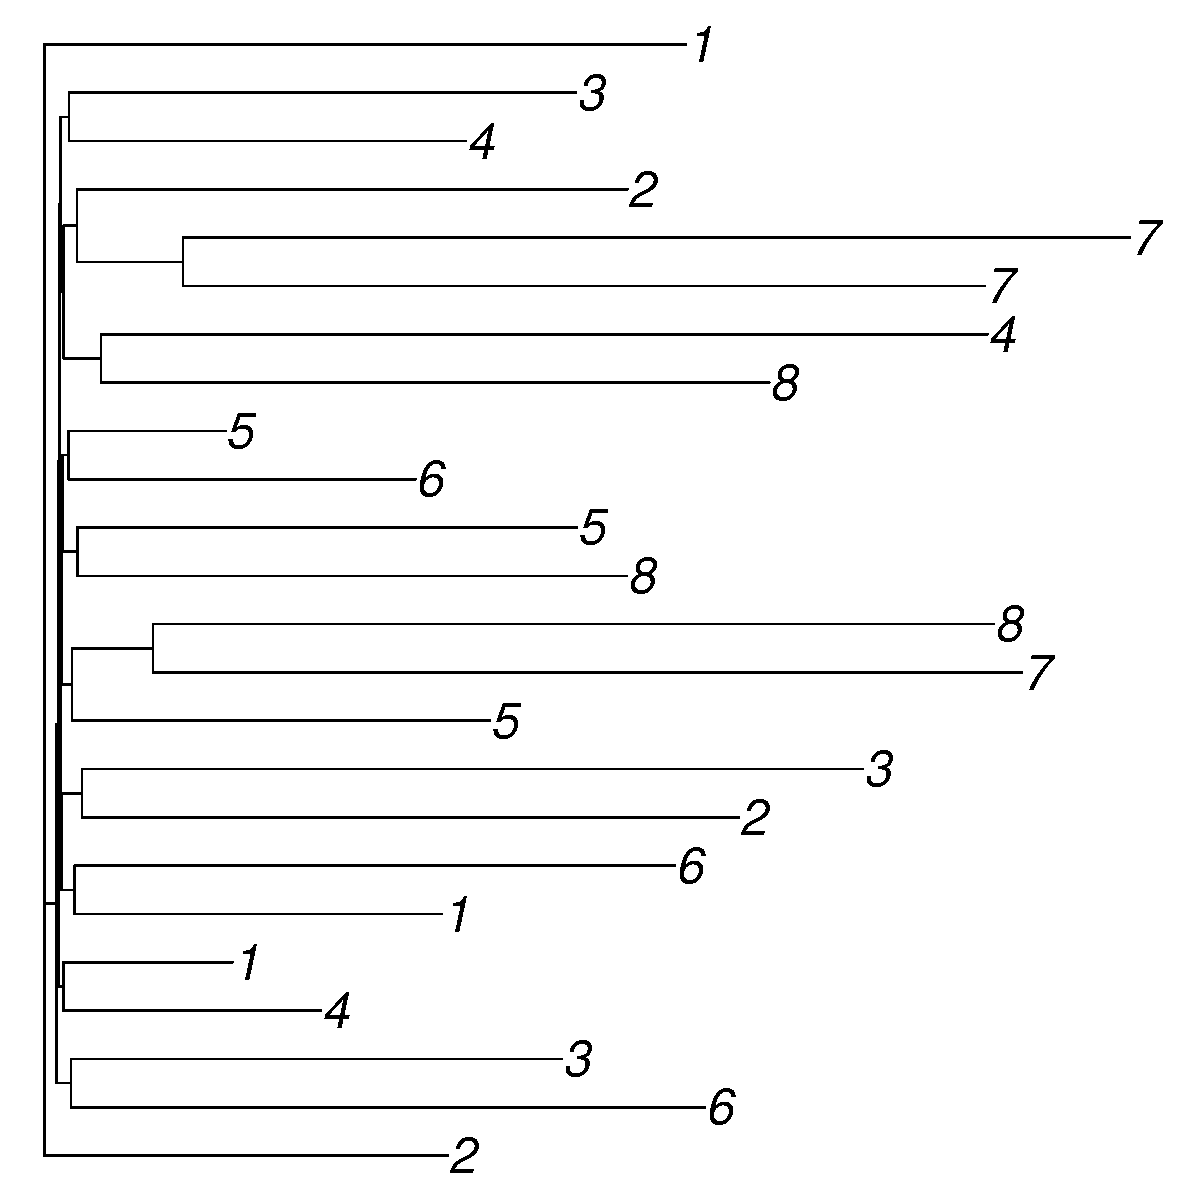
\includegraphics[width=.9\linewidth]{02-depth.pdf} \\
Not within 50bp of an indel & 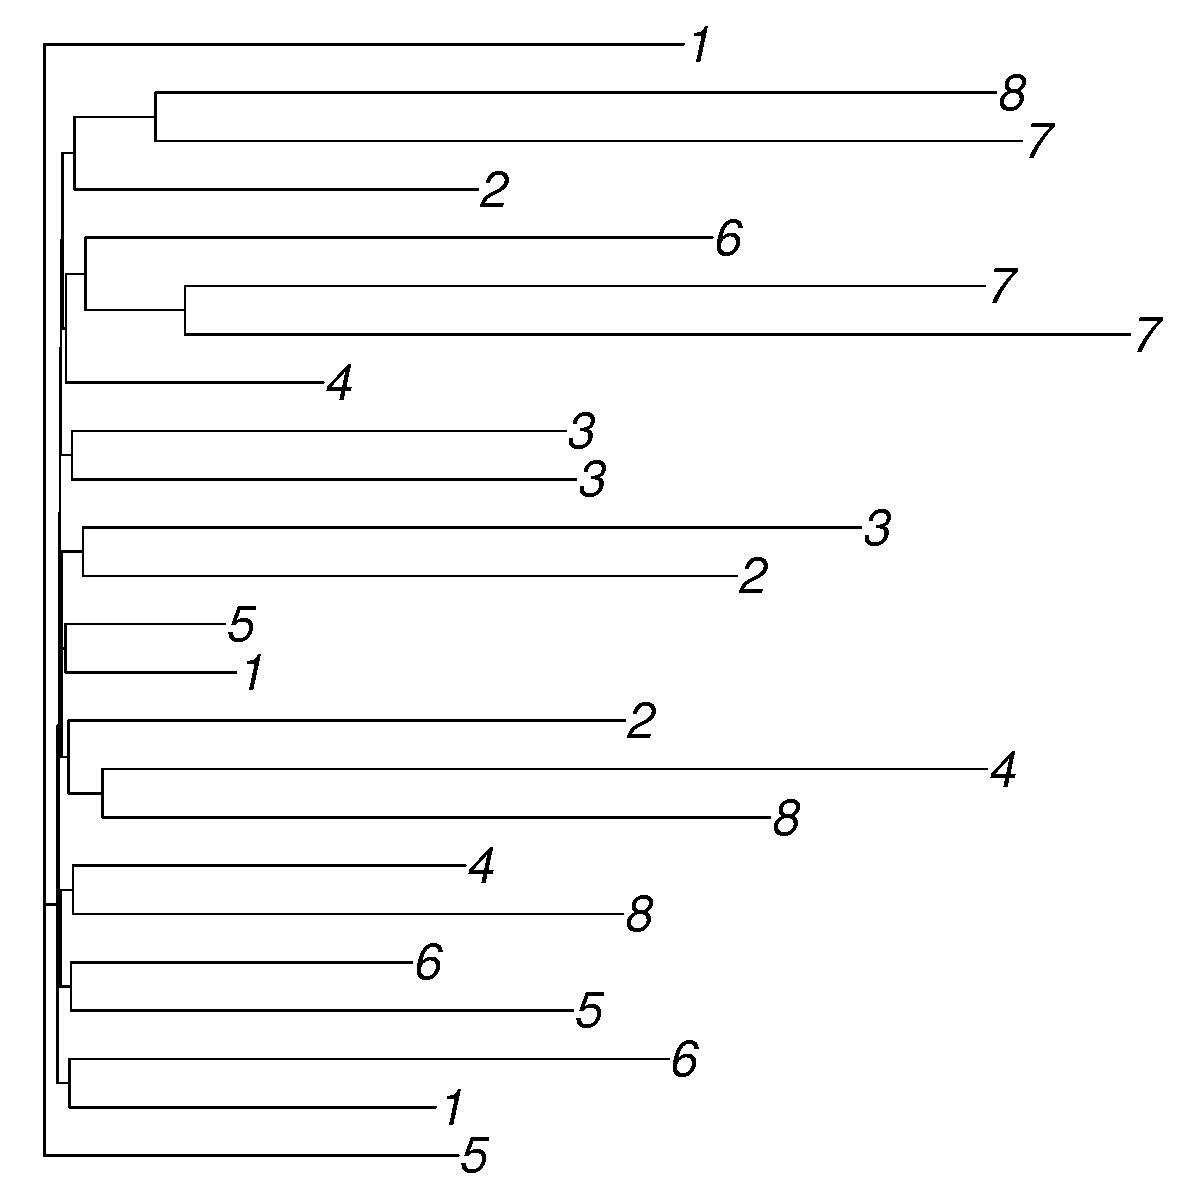
\includegraphics[width=.9\linewidth]{04-near-indel.pdf} \\
% Only variable sites & 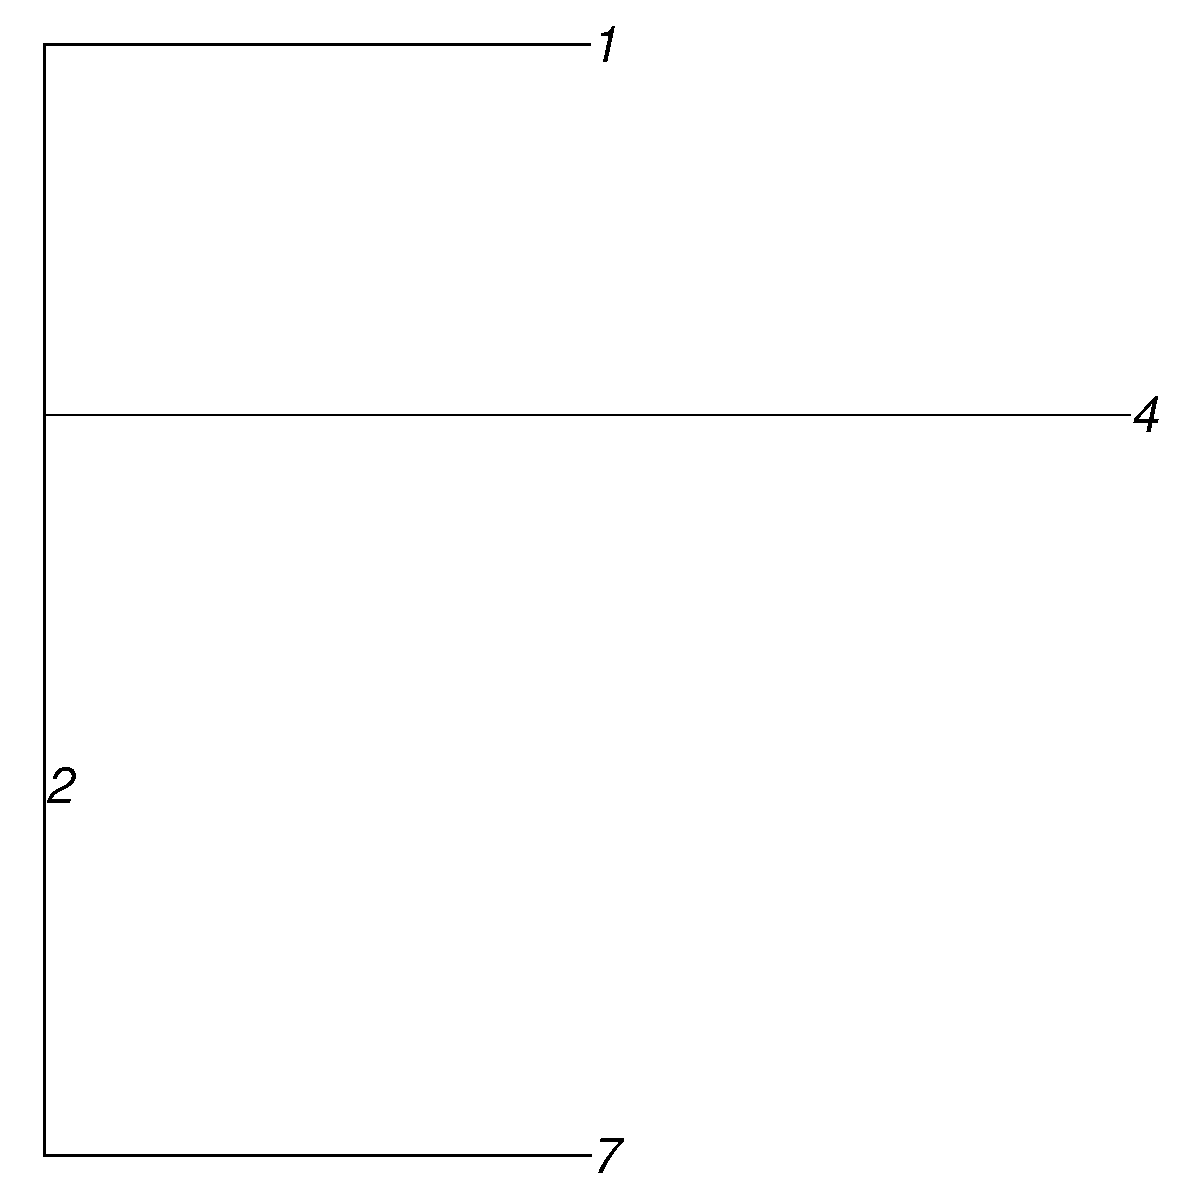
\includegraphics[width=\linewidth]{08-variable.pdf}\\
\bottomrule
\end{tabularx}
\end{figure}

\begin{figure}
% \ContinuedFloat
\centering
\begin{tabularx}{.7\textwidth}{ >{\hsize=.7\hsize\linewidth=\hsize}X >{\hsize=1.3\hsize\linewidth=\hsize}X }
\toprule
Filtering Step & Tree \\
\midrule
Biallelic SNPs & 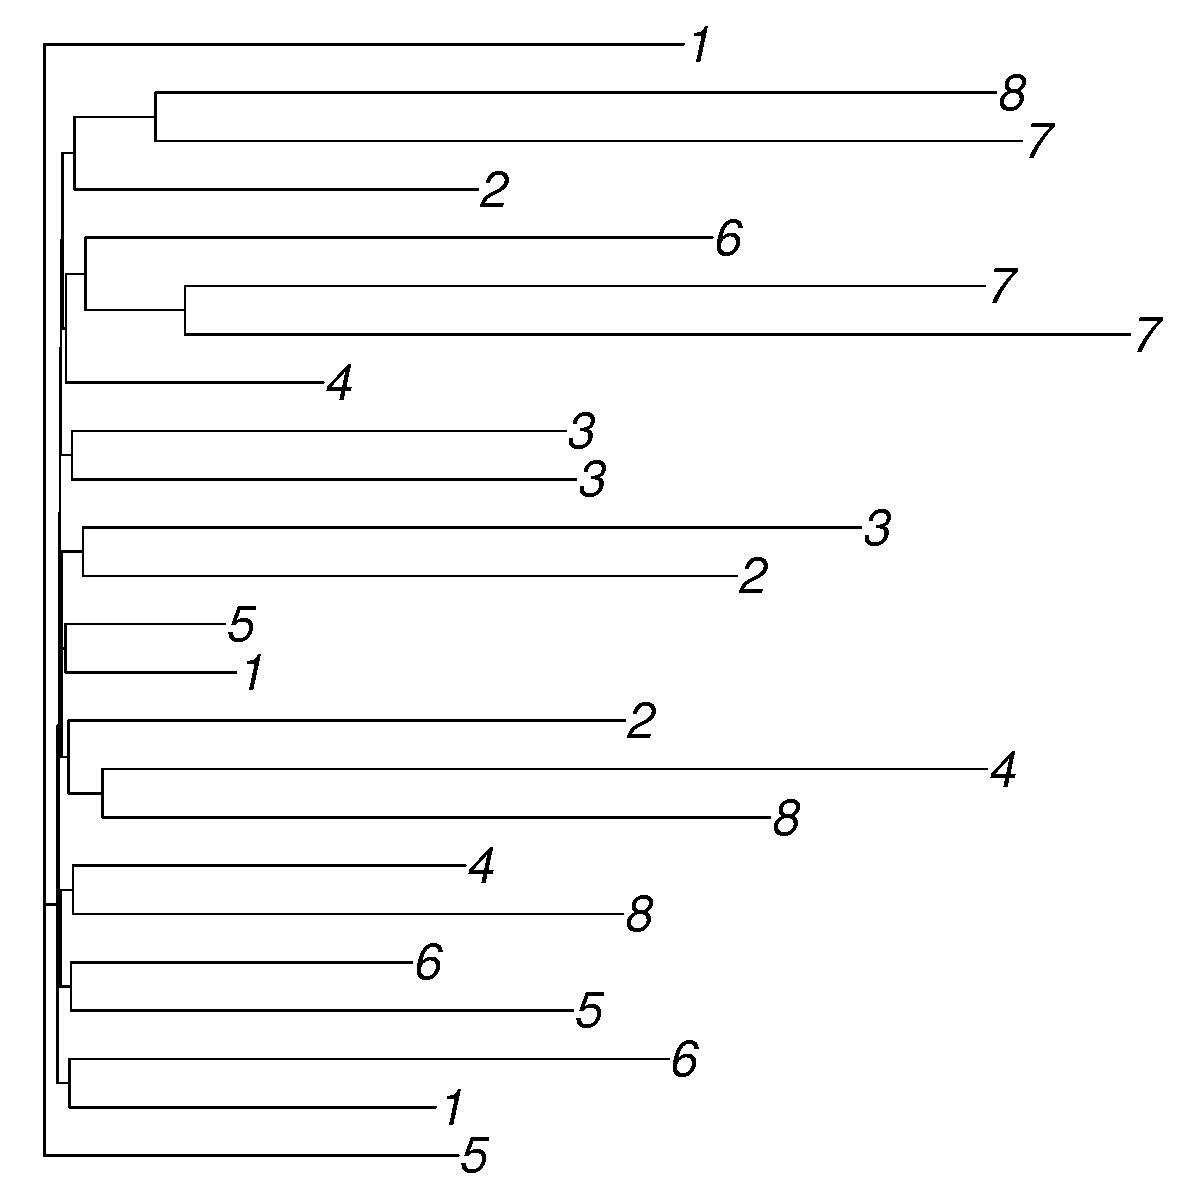
\includegraphics[width=.9\linewidth]{05-biallelic.pdf}\\
Outside repeat \newline regions & 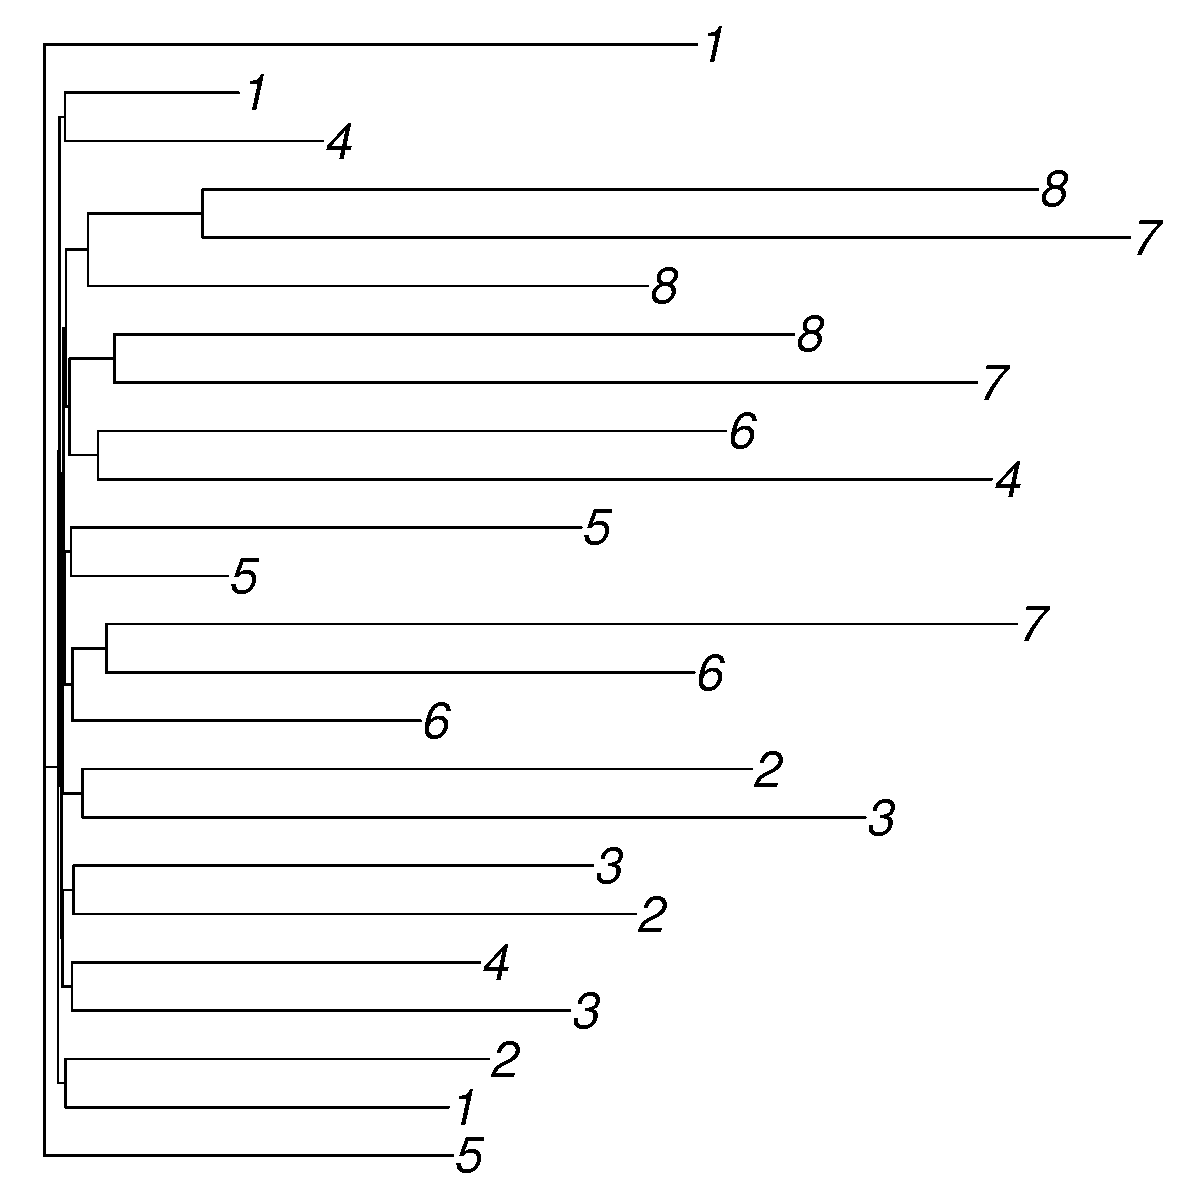
\includegraphics[width=.9\linewidth]{06-repeat.pdf} \\
All 3 replicates match and only variable sites & 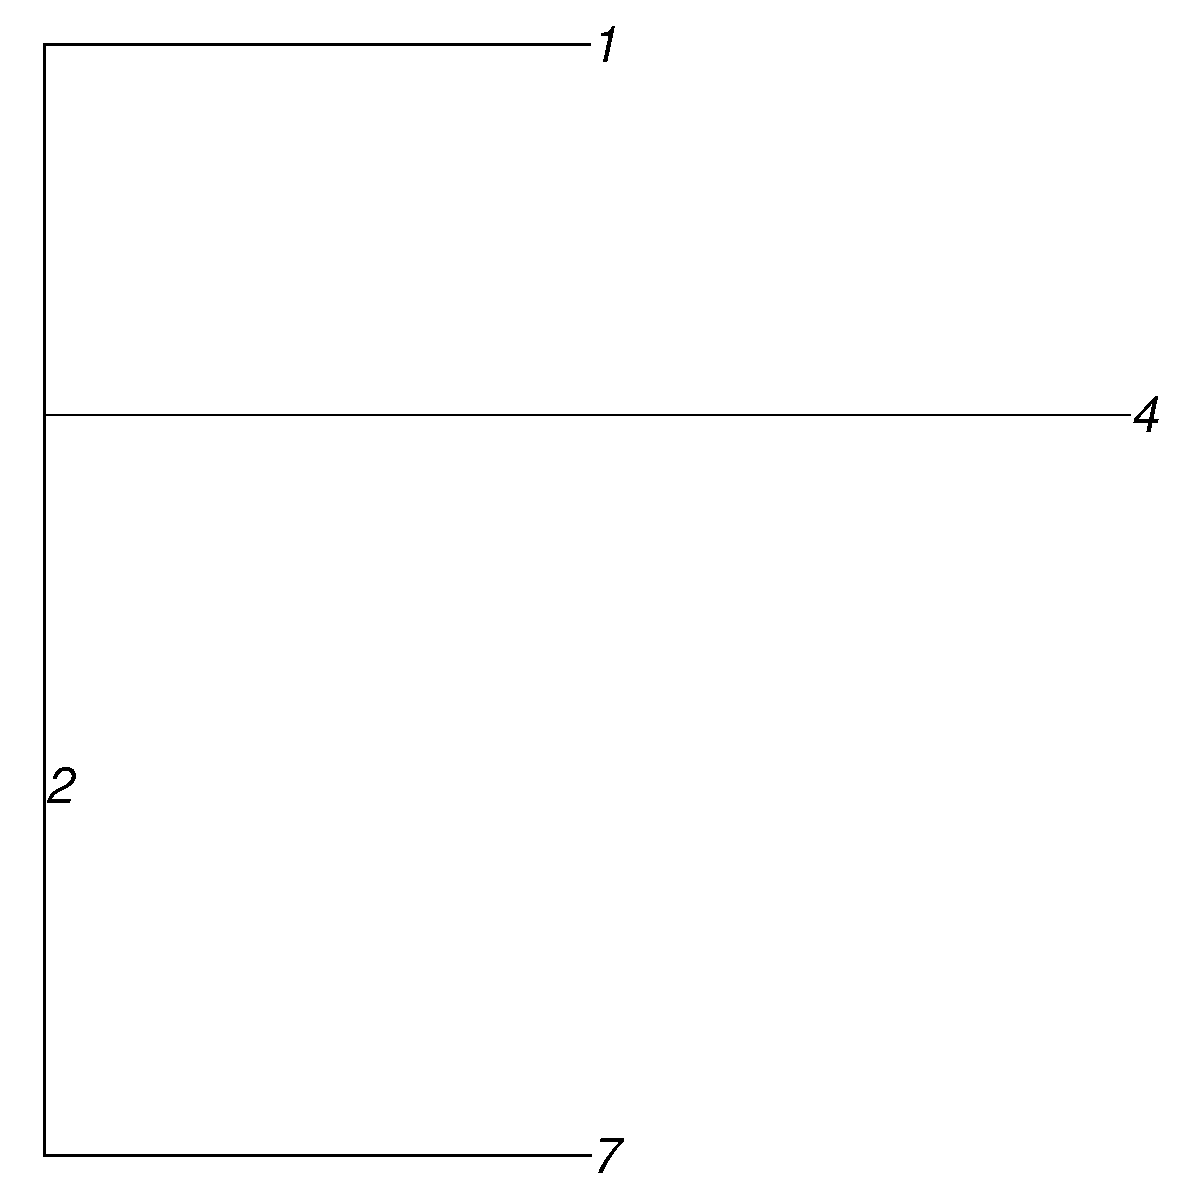
\includegraphics[width=.9\linewidth]{07-replicate.pdf}\\
% Only variable sites & 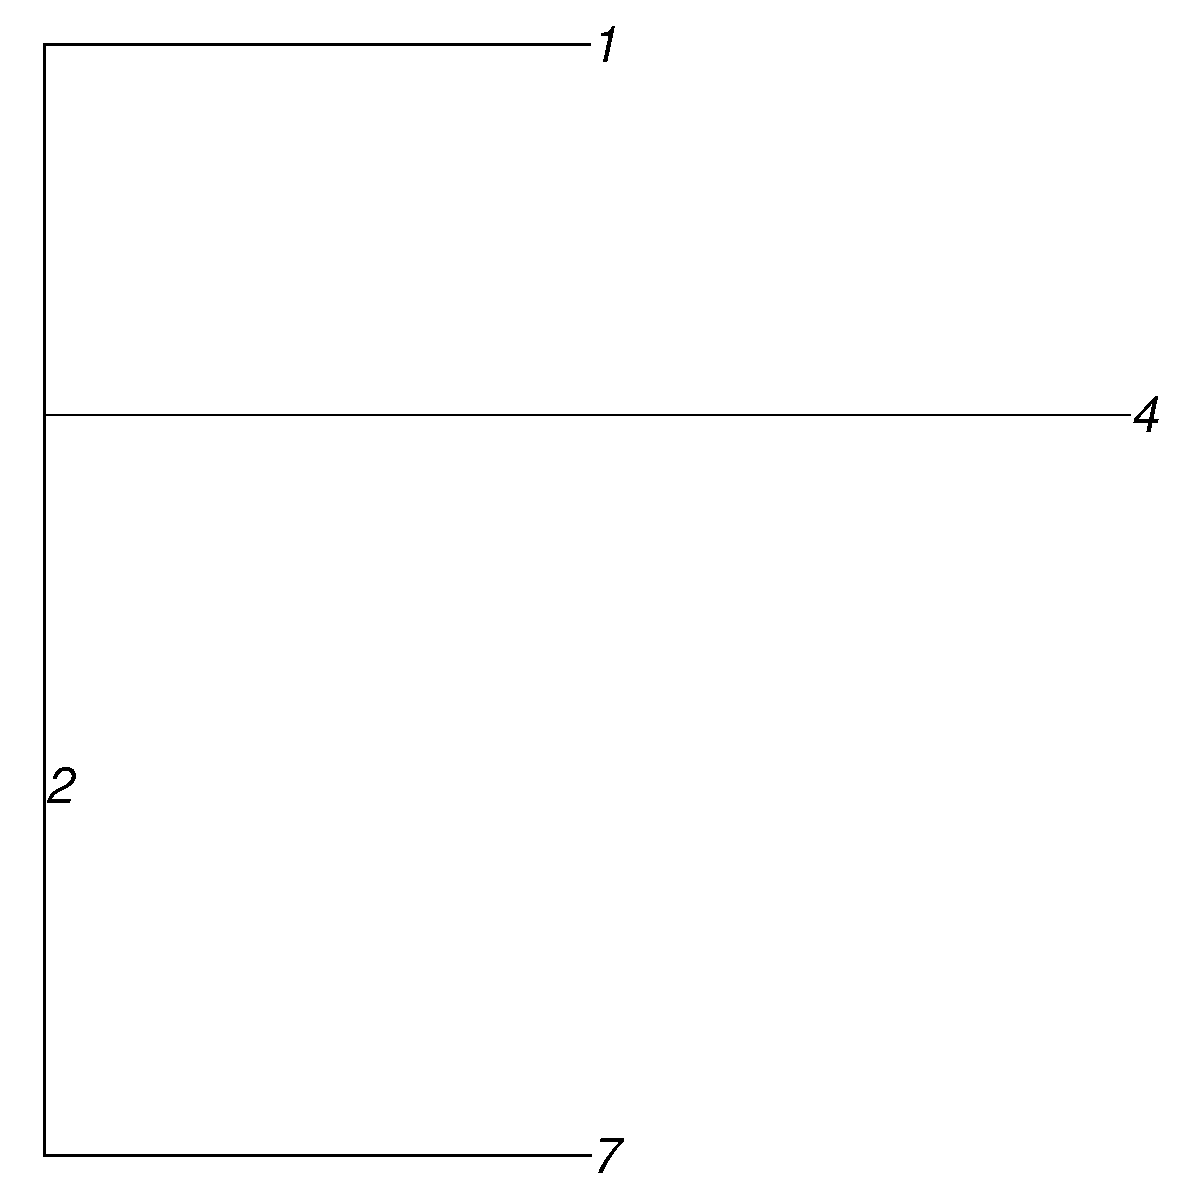
\includegraphics[width=\linewidth]{08-variable.pdf}\\
\bottomrule
\end{tabularx}
\titlecaption{Trees Inferred at Each Filtering Step}{Since each sample was derived from the branch of a tree, its genetic structure should match the physical branching structure. Due to mutations accumulating independently in each branch meristem after branching, the phylogeny should match the true structure.}
\label{fig:ev_filtertrees}
\end{figure}

\section{Discussion}

Based on the trees constructed here (Figure \ref{fig:ev_filtertrees}), DiscoSNP++ was not able to capture the phylogenetic signal in this data. There are many fewer detected variants at the start of the filtering pipeline compared to those in \cite{orr_phylogenomic_2020}, with 951,924 variants on the first 11 scaffolds compared to 9,679,544 detected with HaplotypeCaller. This reduced number of potential variants is consistent throughout filtering steps. In all the constructed trees, replicates of the same sample should cluster closely together; however, this is not the case.

One reason for this is the variant calls emitted by DiscoSNP++ are very sparse, and many sites having at least one missing (./.) genotype (see Table \ref{tbl:ev_missing}). The presence of a missing genotype for any site eliminates the ability for it to contribute useful information during phylogeny construction. Thus, due to the large amount of missing data, the number of informative sites in the alignment is small. 

\begin{table}
\centering
\begin{tabularx}{.8\textwidth}{ l X r }
\toprule
\textbf{Filter} & \textbf{Number of sites with \newline a missing genotype} & \textbf{Percent}\\
\midrule
Appears in first 11 scaffolds & 639441 & 67\\
Total depth <= 500 & 636012 & 70\\
Not within 50bp of an indel & 623544 & 70\\
Biallelic SNPs & 547636 & 67\\
Outside repeat regions & 425544 & 98\\
All 3 replicates match & 309 & 14\\
Only variable sites & 0 & 0\\
\bottomrule
\end{tabularx}
\titlecaption{Number of Sites With a Missing Genotype After Each Filtering Step}{The number of sites with a missing genotype after each filtering step. Many missing genotypes makes it difficult to accurately resolve the tree. In the second to last step, when there are relatively few missing genotypes, there aren't sufficient informative sites to accurately construct the tree.}
\label{tbl:ev_missing}
\end{table}

There are a variety of reasons the algorithm is unable to call genotypes at so many sites. One reason is that the algorithm lacks a reference, so when it detects a variant it may not be able to map it back to the genome. For complex or clustered variants, this may be a sample-specific effect that could contribute to differential calling ability on some samples. This is an especially difficult problem with a repetitive and low-quality genome, such as the one used here. Another major reason is the lack of per-sample depth in this data. Since each replicate was only sequenced to 10X depth, the reads are relatively short, and the genome is repetitive, the de bruijn graph construction may not be well-connected enough to detect variant bubbles.

\section{Conclusion}

Reference-free variant callers have the potential to be powerful tools for detecting variants in non-model organisms. They are also free of reference bias that may impact other variant callers. However, the reference-free caller used here was unable to capture sufficient phylogenetic signal in a structured dataset. Larger per-sample depths and smaller genomes with few repetitive regions would likely improve these results.

\printbibliography[segment=\therefsegment]{}
